\chapter{Teoria}%
\label{ch:teoria}

Tässä kappaleessa käsitellään eri käytettäviä teknologioita perus tasolla.

\section{Stereo Analyysi}

Stereo Analyysillä kuvan käsittelyssä tarkoitetaan kahdesta samasta kohteesta otetusta kuvasta olevien yhtenäisyyksillä syvyyden analysointia. Näiden tietojen avulla voidaan arvioida kuvassa olevien kohteiden etäisyyttä toisistaan sekä kamerasta. Tämä analyysi voidaan suorittaa mille tahansa kahdelle kuvalle eri kuvakulmasta samasta kohteesta. Yleisesti käytettävässä datassa kuitenkin kuvat ovat otettu sivuttais suunnassa vierekkäisistä asemista, ja oletamme että stereokuvamme ovat tällaisia. Tässä tapauksessa kuva datan analysointia helpottaa kuvassa olevien kohteiden asemointi toisiinsa verrattuna, koska niitä ei tarvitse etsiä eri puolilta kuvaa. Tarkan syvyyden laskemisessa onkin kameroiden kalibraation sekä sijainti toisiinsa nähden tarpeellista. Kuitenkin jo pelkästään kahdella kuvalla kohteesta voidaan jo arvioida kohteiden relatiivista etäisyyttä toisiinsa. 

Kuvien pisteiden sijainnin muutosta toisiinsa nähden kutsutaan dispariteetiksi. On erilaisia tekniikoita joilla tämä dispariteetti voidaan arvioida, mutta sen tavoite on löytää sama piste eri kuvista, ja ilmoittaa sen dispariteetti. Jos molemmissa kuvissa tunnistetaan pikseli tai pikselijoukko samassa kohdassa, on sen pisteen dispariteetti nolla, jos ses on siirynyt annetaan sille jokin arvo siirtymäsuunnan mukaan. Kun kuvasta on laskettu haluttu resoluutio tälläisiä pisteitä voidaan siitä generoida 3d pistekartta.

\subsection{SGM Semi global matching}

Jotta stereo analyysi on mahdollista tulee kuvasta tunnistaa samat kohteet. Yksi tapa tehdä tämä tunistanen on Semi-global matchinging avulla\cite{hirschmuller2005babel}. Tämä tekniikka ottaa huomioon pikselin ja sen ympäröpivien pikselien arvot etsiessään toisesta kuvasta vastaavaa arvoa. Tämä sovitus voidaan tehdä kaavalla.

\begin{equation}\label{yht:SGM}
    E(d) = \sum_{p} D(p, d_p) + \sum_{q \in \mathcal{N}} R(p, d_p, q, d_q)
\end{equation}

Tässä kaavassa siis lasketaan yhteen itse pikselin tai pikselialueen dispariteetti \(D(p, d_p)\), sekä valitun joukon sitä ympäröivien pikseleitä samankaltaisuus\(R(p, d_p, q, d_q)\). Näin saadaan arvioitua kustannustehokkaasti samankaltaisuus, koska saman asian ympäröivät pikselit tulisi olla melko samankaltaisia molemmissa kuvissa. 

Eli jos pikseli ja sen ympäriöivät pikselit ovat arvoiltaan saman kaltaisia, on mahdollisuus että ne ovat sama piste kuin verrokki kuvassa. Kun arvo on tarpeeksi suuri voidaan olettaa että kyseessä on sama piste. Näiden pisteiden avulla voidaan arvioida pisteen dispariteetti. Kun pisteen samankaltaisuutta arvioidaan, on usein järkevää käyttää filtereitä odottamattomuuksien ja artifaktien minimoimiseksi. Mutta itse vertailu voidaan tehä vain absoluuttisesti arvoja vertaamalla tai arvo joukon keskiarvoa verraten.

Tämä yhdistetään haluttuun määrään ympäröivien pikselien dispariteettiin. Joiden näin ollen pitäisi olla melko samankaltaisia molemmissa kuvissa. Ja niiden summasta saadaan tulos, josta voidaan yrittää päätellä onko kyseessä sama piste.

Käytetyssä ohjelmakoodissa SGM function implementoinnin hoiti 

"\url{https://docs.opencv.org/3.4/d2/d85/classcv_1_1StereoSGBM.html}"

"\url{https://en.wikipedia.org/wiki/Semi-global_matching}"

\section{Neuroverkot}

Lopulliseen toteutukseen käytetään neuroverkkoa, neuroverkko on yleisesti kuva-analyysiin käytettävä tekniikka, jonka voi kouluttaa datalla niin kuvankäsittelyllisiä kuin muitakin ongelmia. Sen toiminta perustuu neuroneihin joita järjestetään verkkomaiseen rakenteeseen useisiin eri kerroksiin.

\begin{equation}\label{yht:neuroni}
    a = \sigma\left(\sum_i w_i x_i + b\right)
\end{equation}

Tämä on neuronin matemaattinen kaava, se tuottaa ulostulonaan arvon \(a\)  saamiensa syötteiden perusteella. \(x_i\) on neuronin saama syöte. \(w_i\) on neuronille annettu painoarvo. \(b\) on neuronin bias arvo. \(\sigma\) on funktio joka muuttaa neuronin saavan armon välille 0,1.

Kun näitä neuroneita asetetaan eri kerroksiin siten että verkon sisääntulo on esimerkiksi valokuvan kokoinen, ja ulostulo on yhen neuronin ulostulo, voidaan verkolle syöttää kuvia esimerkiksi kissoista ja koirista. Kun näille kuville annetaan arvot 0 ja 1 kuvan aiheen mukaan, voidaan verkko kouluttaa tunnistamaan kissoja ja koiria. Koulutuksen aikana verkko muuttaa arvojaan \(w_i\) ja \(b\). Nämä arvot se saa yrittämällä erilaisia arvoja neuroneille. Kun verkkoa tämän jälkeen testataan on voidaan saaduista lopputuloksista valita paras. Tämän jälkeen tätä lopputulosta voidaan lähteä parantelemaan, testaamalla toimiiko suuremmat vai pienemmät arvot paremmin. Kun näitä kahta arvoa eri neuroneilla muutetaan saadaan paremmin toimiva neuroverkko.

Neuroverkko on siis vain kasa yksinkertaisia matemaattisia funktioita, joiden toimintaa vain tuurilla arvoidaan jotta saadaan haluttu lopputulos. Tätä tuuria pyritään parantamaan ohjaamalla verkon koulutusta. Tämä tapahtuu tappiofunktion (loss function) sekä takaisinvirtausalgoritmin (backpopagation algorithm) avulla. Loss functionin tehtävä on kertoa kuinka paljon saatu tulos eroaa halutusta. Esimerkki tapauksessamme tämä käytännössä katsoisi onko kissa kuvan arvo mikä sen pitäisi olla. Tämän työn lopputulos on verkko joka yrittää luoda kuvasta 3d pistekartan. Siinä tapauksessa siis neliösumma tai jokin muu tapa virheen tunnistamiseen olisi parempi. Kun virhe on tunnistettu verkkoa muokataan takaisinvirtaus algoritmin perusteella. Tähän ei ole yhtä parasta ratkaisua, vaan eri verkkojen ja käyttökohteiden tapauksessa eri algoritmit voivat tuoda huomattavasti parempia tuloksia.

"\url{https://en.wikipedia.org/wiki/Artificial_neural_network}"

\section{Semantic segmentation}

Semantic segmentation eli kuvan segmentointi on yksi yleinen käyttökohde neuroverkoille. Sen avulla on helppo tehdä käytettäviä ja helposti hyödynnettäviä malleja. Esimerkkejä käytöstä on esimerkiksi automatisoidussa liikenteessä erilaisten asioiden erottelu \ref{fig:labels}. Tätä samaa teknologiaa voidaan käyttää useisiin eri applikaatioihin ja se on mahdollisesti yksi parhaita tapoja tarjota tietokoneelle mahdollisimman ihmismäinen tapa tunnistaa asioita kuvista. Näin voidaan yhdestä kuvasta tunnistaa erilaiset löytyvät asiat, esimerkiksi autot, ihmiset tiet puut jne. Samaan asiaan voisi käyttää myös object detection mallia, mutta tunnistustapa on hieman erilainen. Toisinkuin objektin tunnistus joka tunnistaa kuvan alueen missä on esimerkiksi ihminen, segmentointi malli tekee erottelun tarkemmin pikselitasolla.

\begin{figure}
\centering
\pdftooltip{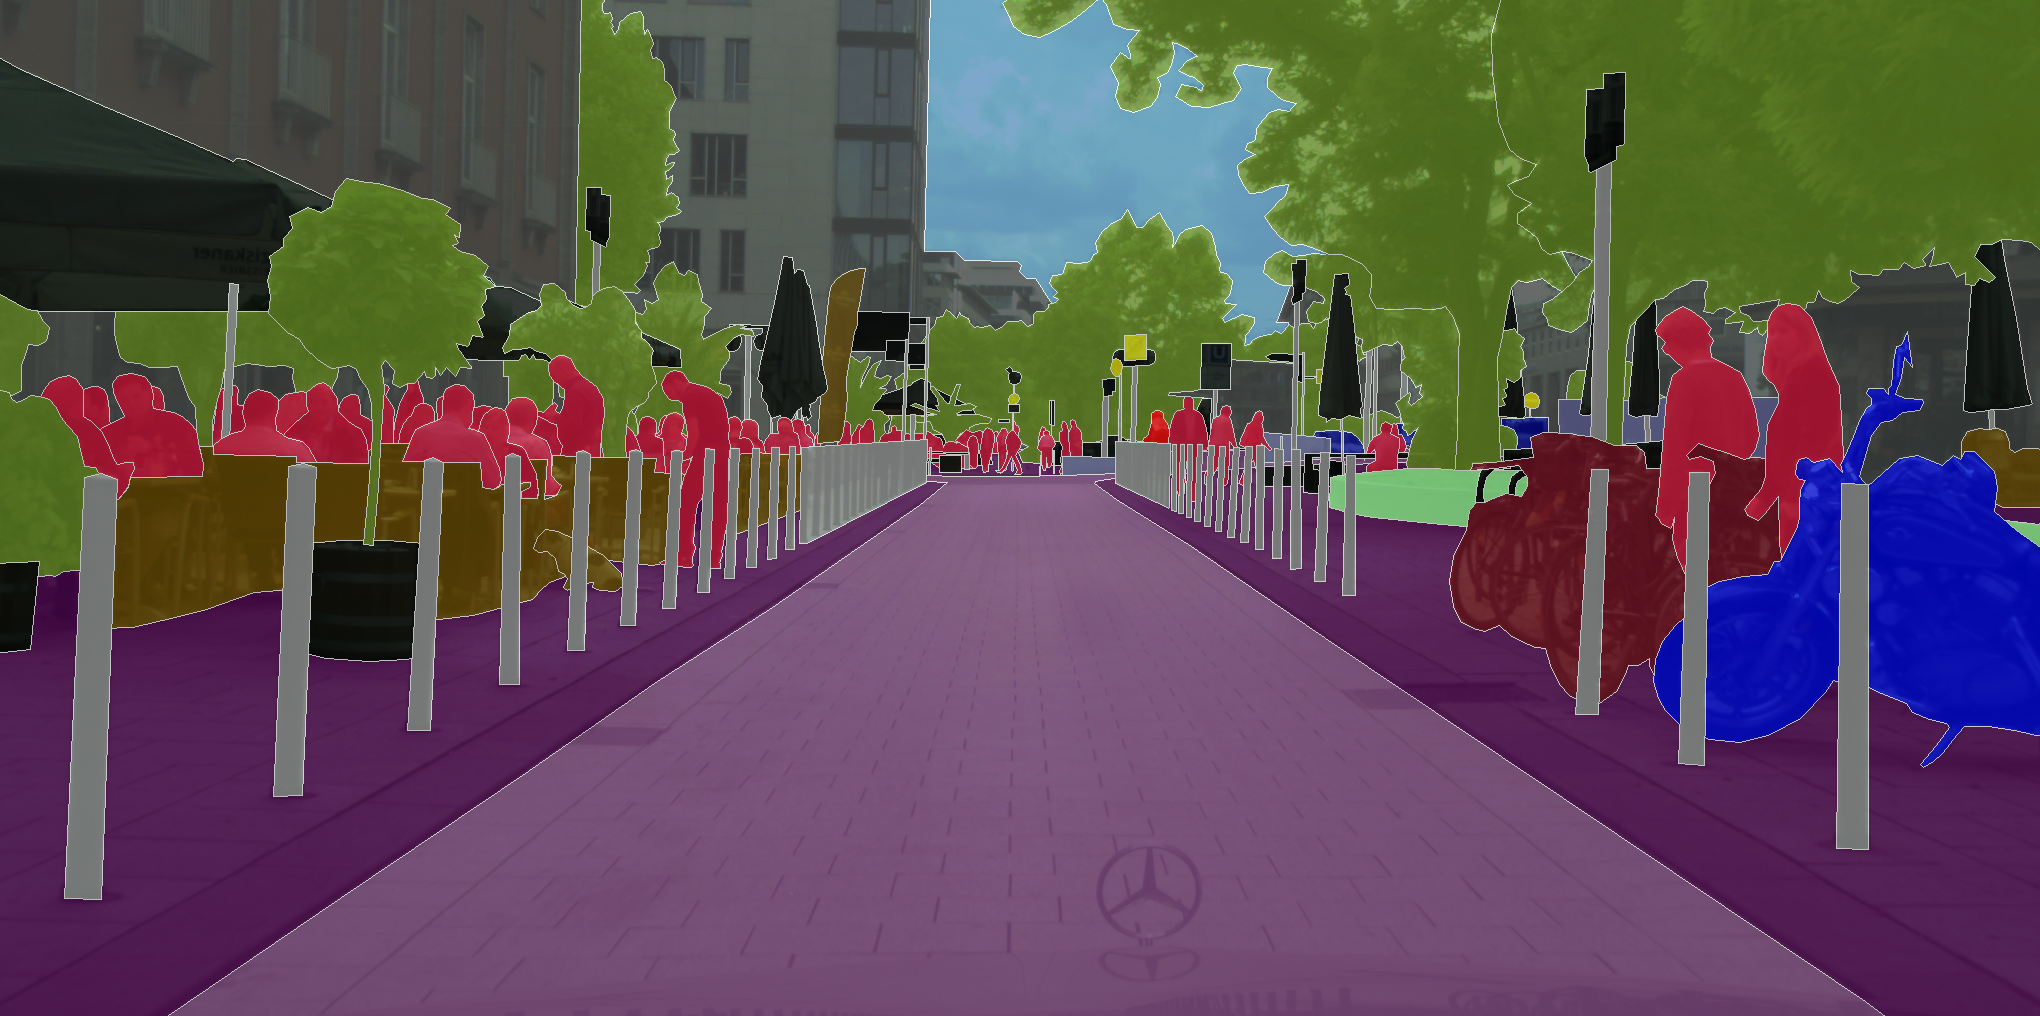
\includegraphics[width=\textwidth]{figures/stuttgart03.png}}{Cityscapes esimerkki kuva stuttgart03}
\caption[Tämä on lyhyt kuvateksti.]{Cityscapes datestin esimerkki segmentointi dataa, jossa kaupunki näkymän erilaiset tunnistattavat kohteet on merkitty eri väreillä.}
\label{fig:labels}
\end{figure}

Kun segmentointi mallin kanssa työskennellään se kuitenkin tuo hieman lisähaastetta datasetin vaatimuksiin koska kuvien pitää olla käsitelty tarkemmin kuin vain varustettuna alueilla missä on asioita. Tämä möyskin hieman muutta tappiofunktion käsittelyä. Koska mallin ei ole tarkoitus palautta pistejoukkoja vaan alueita, ei voida vain verrata ovatko tunnistetut pisteet lähellä koulutuspisteitä, vaan tulee tehdä jonkinnäköistä pinta-alaan perustuvaa analyysiä. 

"Kirjoita lisää"

"\url{https://en.wikipedia.org/wiki/Image_segmentation}"

\section{3d pisteavaruus}

Lopullinen haluttu tuotos on 3d  pisteavaruus. 3d pisteavaruus voidaan ajatella esitetyistä pisteistä joilla on syvyys arvo. Tässä tapauksessa kun pisteavaruus on tehty valokuvien pohjalta, voi myös saadun pisteavaruuden esittää kuvana \ref{fig:depth}. Muissa tilanteissa 3d pisteitä voi kuitenkin sijaita kaksiulotteisesta perspektiivistä katsottuna toistensa takana. Ei siis tule olettaa että kaikki 3d pistekartat on häviöttömästi esitettävissä 2d muodossa. 


\begin{figure}
\centering
\pdftooltip{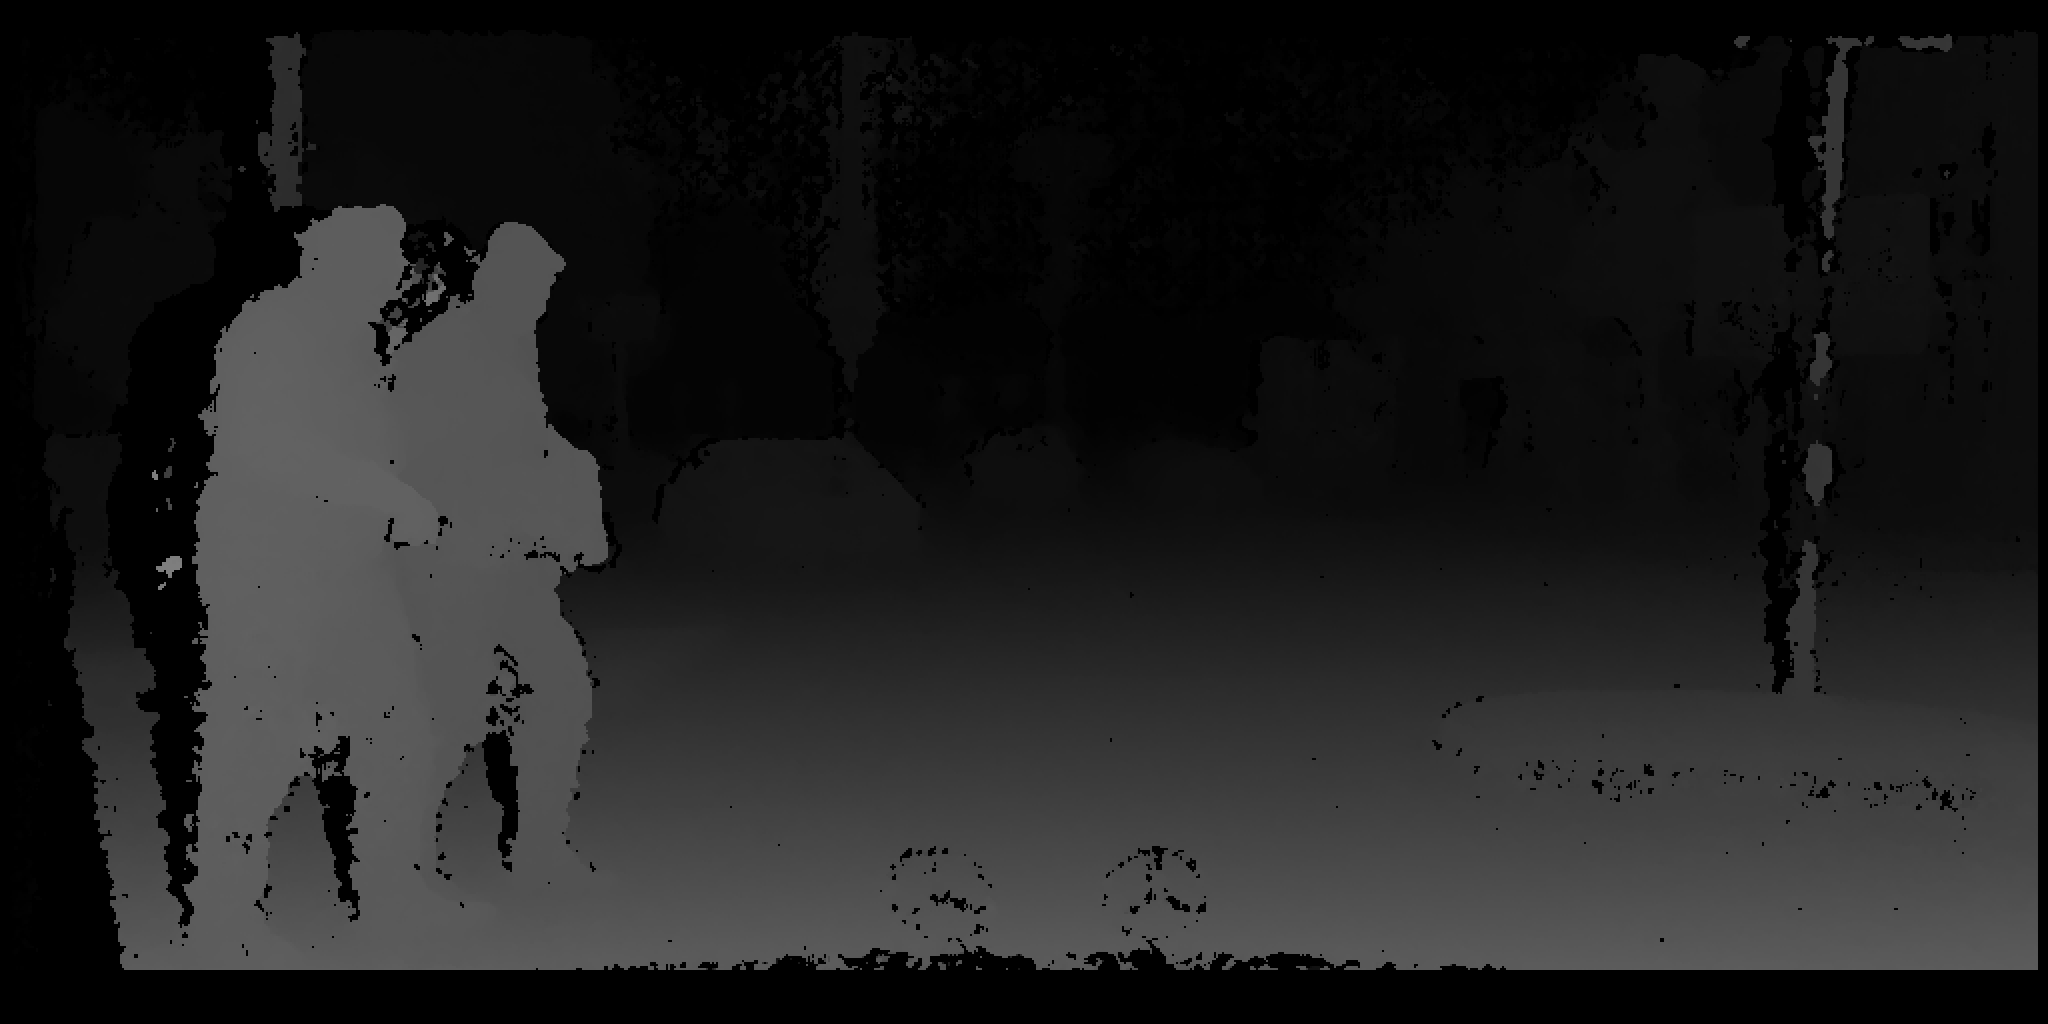
\includegraphics[width=\textwidth]{figures/leverkusen_000024_000019_disparity.png}}{Cityscapes esimerkki kuva leverkusen_000024_000019_disparity}
\caption[Tämä on lyhyt kuvateksti.]{Citysscapes datasetin syvyysdata esimerkki.}
\label{fig:depth}
\end{figure}

3d pistekartat ovat hyvin perusmuotoinen ja epäoptimoitu tapa käsitellä 3d dataa. Jos sitä haluttaisiin optimoida 3d mallin kannattaisi muuttaa kolmioiksi tai muiksi monikulmioiksi joiden perusteella tämä data käsiteltäisiin. Mutta koska edellämainitusti oma datamme voidaan esittää 2d syvyydellisenä kuvana, meillä ei ole tähän tarvetta.

    
"\url{https://en.wikipedia.org/wiki/Point_cloud}"

